
%(BEGIN_QUESTION)
% Copyright 2006, Tony R. Kuphaldt, released under the Creative Commons Attribution License (v 1.0)
% This means you may do almost anything with this work of mine, so long as you give me proper credit

Study this illustration of a simple pneumatic proportional controller:

$$\includegraphics[width=15.5cm]{i01476x01.eps}$$

Answer the following questions about this controller mechanism:

\begin{itemize}
\item{} Is it {\it direct} or {\it reverse} acting?  Annotate the input bellows with ``+'' and ``$-$'' symbols to designate their respective influences on the output signal, just like the input terminals on an operational amplifier.
\vskip 5pt
\item{} Does it work on the {\it force-balance} or {\it motion-balance} principle?
\vskip 5pt
\item{} Explain (step-by-step) what happens when the process variable input signal increases and the setpoint remains the same.
\vskip 5pt
\item{} How could the gain of this controller be increased?
\vskip 5pt
\item{} How could the gain of this controller be decreased?
\vskip 5pt
\item{} How could the bias of this controller be adjusted?
\vskip 5pt
\item{} How could the direction of action (direct vs. reverse) be changed?
\end{itemize}

\vskip 20pt \vbox{\hrule \hbox{\strut \vrule{} {\bf Suggestions for Socratic discussion} \vrule} \hrule}

\begin{itemize}
\item{} The distinction between force-balance and motion-balance is one that tends to confuse students.  A common tactical error students make is to attempt to memorize distinguishing characteristics in order to identify what type of balancing a particular mechanism employs.  A better approach is to {\it think through} the operation of such pneumatic mechanisms using ``thought experiments'' to identify which balance principle they employ.  Why do you think it is bad to go with the memorization approach instead of the ``thought experiment'' approach?
\item{} What difference does it make to us (as technicians) to know whether a mechanism is force- or motion-balance?  In other words, who cares???
\end{itemize}

\underbar{file i01476}
%(END_QUESTION)





%(BEGIN_ANSWER)

\noindent
{\bf Partial answer:}

\begin{itemize}
\item{} Does it work on the {\it force-balance} or {\it motion-balance} principle? {\bf Force-balance} (actually, it is a {\it moment-balance} mechanism, to be precise).
\vskip 5pt
\item{} Explain (step-by-step) what happens when the process variable input signal increases and the setpoint remains the same. {\bf First, the baffle moves away from the nozzle, decreasing backpressure, decreasing force exerted by the feedback bellows, returning the system to equilibrium with a lesser output pressure}.
\vskip 5pt
\item{} How could the bias of this controller be adjusted? {\bf Change the spring tension}.
\end{itemize}

$$\includegraphics[width=15.5cm]{i01476x02.eps}$$

%(END_ANSWER)





%(BEGIN_NOTES)

\begin{itemize}
\item{} Is it {\it direct} or {\it reverse} acting? {\bf Reverse-acting}
\vskip 5pt
\item{} Does it work on the {\it force-balance} or {\it motion-balance} principle? {\bf Force-balance} (actually, it is a {\it moment-balance} mechanism, to be precise).
\vskip 5pt
\item{} Explain (step-by-step) what happens when the process variable input signal increases and the setpoint remains the same. {\bf First, the baffle moves away from the nozzle, decreasing backpressure, decreasing force exerted by the feedback bellows, returning the system to equilibrium with a lesser output pressure}.
\vskip 5pt
\item{} How could the gain of this controller be increased? {\bf By moving the fulcrum closer to the feedback bellows}.
\vskip 5pt
\item{} How could the gain of this controller be decreased? {\bf By moving the fulcrum further away from the feedback bellows}.
\vskip 5pt
\item{} How could the bias of this controller be adjusted? {\bf Change the spring tension}.
\vskip 5pt
\item{} How could the direction of action (direct vs. reverse) be changed?  {\bf Reverse the PV and SP inputs, so that both signals go to the opposite bellows they do now}.
\end{itemize}

\vskip 10pt

Students often get their answers reversed for increasing/decreasing controller gain, because they tend to think in terms of motion rather than force.  In other words, some students will say that to increase gain you must move the fulcrum further away from the baffle/nozzle and feedback bellows because that will yield greater motion for any given change in input (PV or SP) signal.  However, this is incorrect because it is not motion that determines output in this controller, but rather force.  The fulcrum must be moved closer to the feedback bellows for more gain because this is what will place the feedback bellows in a position of less mechanical advantage, so it must ``fight back'' harder to balance any given change in input pressure(s).








\filbreak \vskip 20pt \vbox{\hrule \hbox{\strut \vrule{} {\bf Virtual Troubleshooting} \vrule} \hrule}

\noindent
{\bf Predicting the effect of a given fault:} present each of the following faults to the students, one at a time, having them comment on all the effects each fault would produce.

\begin{itemize}
\item{} Nozzle plugs
\item{} Restriction plugs
\item{} Tube between output line and output bellows plugs
\item{} Spring breaks
\item{} Output bellows develops a leak
\item{} SP bellows develops a leak
\item{} PV bellows develops a leak
\item{} Baffle gets bent upward on beam (away from nozzle)
\item{} Supply air pressure increases
\item{} Supply air pressure decreases
\end{itemize}











\vfil \eject

\noindent
{\bf Prep Quiz:}

Determine what will happen if the process variable signal suddenly increases (e.g. jumps from 5 PSI to 7 PSI in a fraction of a second) in this pneumatic controller mechanism:

$$\includegraphics[width=15.5cm]{i01476x01.eps}$$

\begin{itemize}
\item{} The output signal pressure will suddenly increase 
\vskip 5pt 
\item{} The output signal pressure will gradually decrease over time
\vskip 5pt 
\item{} The setpoint signal pressure will suddenly decrease 
\vskip 5pt 
\item{} The output signal pressure will gradually increase over time 
\vskip 5pt 
\item{} The setpoint signal pressure will suddenly increase
\vskip 5pt 
\item{} The output signal pressure will suddenly decrease 
\end{itemize}


\vfil \eject

\noindent
{\bf Prep Quiz:}

Determine what will happen if the process variable signal suddenly decreases (e.g. jumps from 7 PSI to 5 PSI in a fraction of a second) in this pneumatic controller mechanism:

$$\includegraphics[width=15.5cm]{i01476x01.eps}$$

\begin{itemize}
\item{} The output signal pressure will suddenly increase 
\vskip 5pt 
\item{} The output signal pressure will gradually decrease over time
\vskip 5pt 
\item{} The setpoint signal pressure will suddenly decrease 
\vskip 5pt 
\item{} The output signal pressure will gradually increase over time 
\vskip 5pt 
\item{} The setpoint signal pressure will suddenly increase
\vskip 5pt 
\item{} The output signal pressure will suddenly decrease 
\end{itemize}


%INDEX% Control, proportional: pneumatic force-balance controller

%(END_NOTES)


